\fbox{\begin{minipage}[t]{0.45\textwidth}
    \scriptsize
    \textbf{\scriptsize Linked List}\\
        \scriptsize
        Linear data structure where each node contains: \\
        1. \textbf{key/data}: The value stored in the node \\
        2. \textbf{next}: A pointer to the next node in the sequence \\
        3. \textbf{prev}: A pointer to the previous node (in doubly linked lists) \\
    \textbf{\scriptsize List-Search (find a node with a given key)}\\
    \begin{minipage}[htp]{0.65\textwidth}
        \scriptsize
        1. Start from the head of the linked list.\\
        2. Traverse the list by following the next pointers.\\
        3. Compare each node's key with the target key.\\
        4. Return the node if the key is found.\\
        5. Return NULL if the end of the list is reached without finding the key.
    \end{minipage}
    \begin{minipage}[htp]{0.3\textwidth}
        \begin{center}
            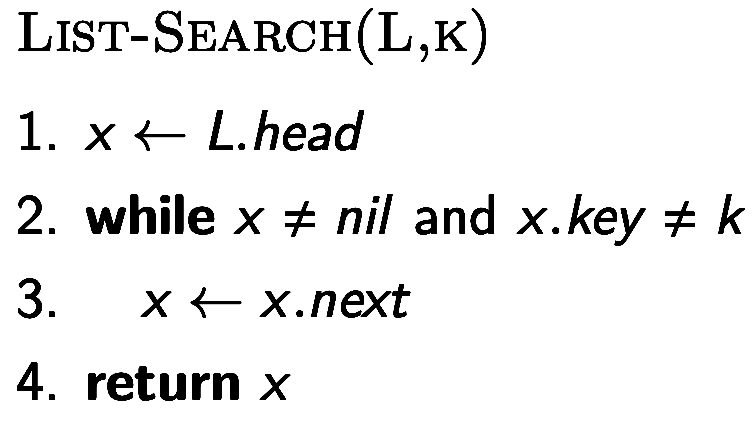
\includegraphics[width=1.1\textwidth]{images/list-search.png}
        \end{center}
    \end{minipage}\\
    \textit{Time Complexity:} \(O(n)\) where n is list length \quad \textit{Space Complexity:} \(O(1)\)\\
    \textbf{\scriptsize List-Insert (insert a new node at the beginning)}\\
    \begin{minipage}[htp]{0.65\textwidth}
        \scriptsize
        1. Create a new node with the given key.\\
        2. Set the next pointer of the new node to point to the current head.\\
        3. If implementing a doubly linked list, set the prev pointer of the current head to the new node.\\
        4. Update the head pointer to point to the new node.\\
        5. If the list was empty, update the tail pointer as well.
    \end{minipage}
    \begin{minipage}[htp]{0.3\textwidth}
        \begin{center}
            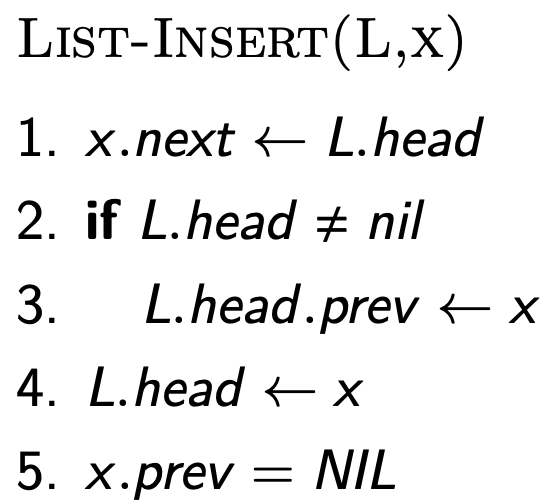
\includegraphics[width=0.9\linewidth]{images/list-insert.png}
        \end{center}
    \end{minipage}\\
    \textit{Time Complexity:} \(O(1)\) \quad \textit{Space Complexity:} \(O(1)\)\\
    \textbf{\scriptsize List-Delete \\(remove a node from the list)}\\
    \begin{minipage}[htp]{0.65\textwidth}
        \scriptsize
        1. Find the node to be deleted (may require traversal).\\
        2. If the node is the head, update the head pointer to the next node.\\
        3. Otherwise, update the next pointer of the previous node to skip the node being deleted.\\
        4. For doubly linked lists, also update the prev pointer of the next node.\\
        5. Free the memory allocated for the deleted node.\\
        6. Handle edge cases: empty list, deleting the only node, or deleting the tail.
    \end{minipage}
    \begin{minipage}[htp]{0.3\textwidth}
        \begin{center}
            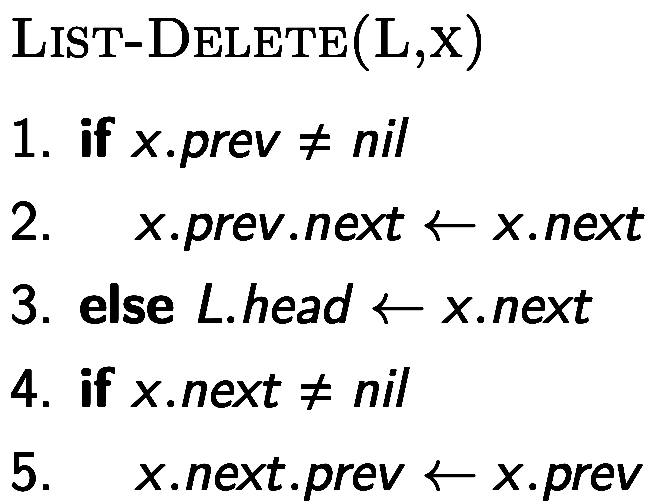
\includegraphics[width=0.9\linewidth]{images/list-delete.png}
        \end{center}
    \end{minipage}\\
    \textit{Time Complexity:} \(O(n)\) for finding the node, \(O(1)\) for deletion \\ \textit{Space Complexity:} \(O(1)\)
\end{minipage}} 